% !TEX program = xelatex
\documentclass[a4paper]{article}
\usepackage{amssymb}   
\usepackage[dvipsnames]{xcolor}
\usepackage{stmaryrd} % 引入 stmaryrd 包以使用 \rrbracket
\usepackage{ctex}
% \usepackage[utf8]{inputenc}
\usepackage{multirow}
\usepackage{graphicx}  % 插图

% \usepackage{mathrsfs}  % 数学字体
\usepackage{enumitem}  % 列表
\usepackage{geometry}  % 页面调整
% \usepackage{unicode-math}
\usepackage[colorlinks,linkcolor=black]{hyperref}
\usepackage{booktabs,tabularx,multicol} % 制表格
\usepackage{amsmath}
% \usepackage{stmaryrd}
\usepackage{amsthm}
\usepackage{amsfonts}
% \usepackage{amssymb}
\usepackage{physics}
\usepackage{appendix}
\usepackage{subfig,graphicx}    % 插入照片
\usepackage{float}      % 固定浮动体
\usepackage{lipsum,zhlipsum} %生成一些测试文本
\usepackage{soul}

\usepackage{algorithm}
\usepackage{algorithmic}

% \usepackage{bm}
\numberwithin{equation}{section}
% 页码设置
\geometry{top=25.4mm,bottom=25.4mm,left=15mm,right=15mm,headheight=2.17cm,headsep=4mm,footskip=12mm}

\usepackage{listings,matlab-prettifier} % MATLAB 美化包
\lstset{
        style=Matlab-editor,
        numbers      = left,
        frame        = single,
}

% 设置列表环境的上下间距
\setenumerate[1]{itemsep=5pt,partopsep=0pt,parsep=\parskip,topsep=5pt}
\setitemize[1]{itemsep=5pt,partopsep=0pt,parsep=\parskip,topsep=5pt}
\setdescription{itemsep=5pt,partopsep=0pt,parsep=\parskip,topsep=5pt}

% 定理环境
% ########## 定理环境 start ####################################


% #### 将 config.tex 中的定理环境的对应部分替换为如下内容
% 定义单独编号,其他四个共用一个编号计数 这里只列举了五种,其他可类似定义(未定义的使用原来的也可)
\usepackage{tcolorbox}
\tcbuselibrary{most}

\newtcbtheorem[number within=section]{defn}%
{定义}{colback=OliveGreen!10,colframe=Green!70,fonttitle=\bfseries}{def}

\newtcbtheorem[number within=section]{lemma}%
{引理}{colback=Salmon!20,colframe=Salmon!90!Black,fonttitle=\bfseries}{lem}

% 使用另一个计数器 use counter from=lemma
\newtcbtheorem[use counter from=lemma, number within=section]{them}%
{定理}{colback=SeaGreen!10!CornflowerBlue!10,colframe=RoyalPurple!55!Aquamarine!100!,fonttitle=\bfseries}{them}

\newtcbtheorem[use counter from=lemma, number within=section]{criterion}%
{准则}{colback=green!5,colframe=green!35!black,fonttitle=\bfseries}{cri}

\newtcbtheorem[use counter from=lemma, number within=section]{corollary}%
{推论}{colback=Emerald!10,colframe=cyan!40!black,fonttitle=\bfseries}{cor}

\newtheorem{remark}{Remark}
\newtheorem{example}{Example}
\newtheorem{proposition}{Proposition}
\newtheorem{theorem}{Theorem}
\newtheorem{definition}{Definition}


% ######### 定理环境 end  #####################################

% ↓↓↓↓↓↓↓↓↓↓↓↓↓↓↓↓↓ 以下是自定义的命令  ↓↓↓↓↓↓↓↓↓↓↓↓↓↓↓↓


\newcommand{\bm}[1]{\boldsymbol{#1}}    % 加粗,常用于向量
\title{求解线性方程组的迭代方法结课报告}
\author{xxxxxx}
\date{\today}
\begin{document}
\maketitle

\section{基础知识}
% \begin{definition}
%     如果  $\boldsymbol{A}$  的元素满足
%     \begin{equation}
%         \left|a_{i i}\right|>\sum_{\substack{i=1 \\ j \neq i}}^{n}\left|a_{i}\right|, \quad i=1,2, \cdots, n,
%     \end{equation}
%     称  $A$  为严格对角占优矩阵. 如果  $\boldsymbol{A}$  的元素满足
%     \begin{equation}
%         \left|a_{i i}\right| \geqslant \sum_{\substack{j=1 \\ j \neq i}}^{n}\left|a_{i j}\right|, \quad i=1,2, \cdots, n,
%     \end{equation}
%     且上式至少有一个不等式严格成立, 则称 $A$ 为弱对角占优矩阵.
% \end{definition}

令  $\bm{x}_{a}$  是线性方程组  $\bm{A x}=\bm{b}$  的近似解. 余项是向量  $\bm{r}=\bm{b}-\bm{A x}_{a}$. 后向误差是余项的范数  $\left\|\bm{b}-\bm{A x}_{a}\right\|_{\infty}$ , 前向误差是  $\left\|\bm{x}-\bm{x}_{a}\right\|_{\infty}$.相对后向误差为 $\frac{\|\bm{r}\|_{\infty}}{\|\bm{b}\|_{\infty}}$ 相对前向误差定义为 $\frac{\left\|\bm{x}-\bm{x}_{a}\right\|_{\infty}}{\|\bm{x}\|_{\infty}}$. 方程  $\bm{A x}=\bm{b}$ 的误差放大因子是二者的比率, 即:
\begin{equation}
    \text { 误差放大因子 }=\frac{\text { 相对前向误差 }}{\text { 相对后向误差 }}=\frac{\left\|\bm{x}-\bm{x}_{a}\right\|_{\infty}}{\|\bm{x}\|_{\infty}} \bigg/ \frac{\|\bm{r}\|_{\infty}}{\|\bm{b}\|_{\infty}}
\end{equation}


方阵  $\bm{A}$  的条件数  $\operatorname{cond}(\bm{A})$  为求解  $\bm{Ax} =\bm{b}$  时, 对于所有右侧向量  $\bm{b}$, 可能出现的最大误差放大因子. 可以证明, $n \times n$  矩阵  $A$  的条件数是
\begin{equation}
    \operatorname{cond}(\bm{A})=\|\bm{A}\|_\infty \cdot\left\|\bm{A}^{-1}\right\|_\infty
\end{equation}
其中 $\left\|\bm{A}\right\|_{\infty }=\max \limits _{1\leq i\leq n}\sum _{j=1}^{n}|a_{ij}|$.

条件数的大小对求解线性方程组的影响是巨大的,一个著名的例子是希尔伯特矩阵.希尔伯特矩阵 $\bm{H}$ 的元素是  $\bm{H}_{i j}=1 /(i+j-1)$, 其对应的条件数非常大. 记 $\bm{H}_6$ 为六阶的希尔伯特矩阵,$\bm{b}_6=\bm{H} \cdot[1, \cdots, 1]^{\mathrm{T}}$,此时的条件数约为 $10^7$. 使用 MATLAB 的 $\backslash$ 命令计算  $\bm{H}_{6}\bm{x}=\bm{b}_6$ 的解, 其计算结果大约有9位正确的位数.对于10阶的情况,条件数约为 $10^{13}$,此时正确位数只有3位了.值得强调的是,MATLAB 的 $\backslash$ 命令是世界上广为流行的先进的线性方程组的求解方法之一,尽管如此,计算结果仍不令人满意.
\section{代求方程}
考虑线性方程组
\begin{equation}
    \label{equ:targetEquation}
    Ax=b,
\end{equation}
其中矩阵 $A$ 的主对角线元素 $a_{i,i}=i,\,,(i=1,2,\cdots,n)$, $A$ 上二对角线和下二对角线的元素均为 $0.5$,向量 $b$ 是矩阵$A$与一个$n$行1列全1向量相乘的结果.例如,对于 $n=10$ 的情况,上述方程组可以表示为:
\begin{equation}
    \begin{bmatrix}
        1   & 0.5 & 0.5 &     &     &     &     &     &     &     \\
        0.5 & 2   & 0.5 & 0.5 &     &     &     &     &     &     \\
        0.5 & 0.5 & 3   & 0.5 & 0.5 &     &     &     &     &     \\
            & 0.5 & 0.5 & 4   & 0.5 & 0.5 &     &     &     &     \\
            &     & 0.5 & 0.5 & 5   & 0.5 & 0.5 &     &     &     \\
            &     &     & 0.5 & 0.5 & 6   & 0.5 & 0.5 &     &     \\
            &     &     &     & 0.5 & 0.5 & 7   & 0.5 & 0.5 &     \\
            &     &     &     &     & 0.5 & 0.5 & 8   & 0.5 & 0.5 \\
            &     &     &     &     &     & 0.5 & 0.5 & 9   & 0.5 \\
            &     &     &     &     &     &     & 0.5 & 0.5 & 10  \\
    \end{bmatrix}
    \begin{bmatrix}
        x_1    \\
        x_2    \\
        x_3    \\
        x_4    \\
        x_5    \\
        x_6    \\
        x_7    \\
        x_8    \\
        x_9    \\
        x_{10} \\
    \end{bmatrix}
    =
    \begin{bmatrix}
        2    \\
        3.5  \\
        5    \\
        6    \\
        7    \\
        8    \\
        9    \\
        10   \\
        10.5 \\
        11   \\
    \end{bmatrix}
\end{equation}
可以证明,矩阵 $A$ 是正定的,此外,当$n=1000$ 时,矩阵 $A$ 的条件数为1.3563e+03,这表明 $A$ 是病态矩阵.

\section{三种基础迭代方法}
令 $D$ 表示 $A$ 的主对角线矩阵, $L$ 表示矩阵  $A$ 的下三角矩阵 (主对角线以下的元素), $U$ 表示上三角矩阵 (主对角线以上的元素), 则  $A=L+D+U$, 求解的方程变为  $L x+D x+U x=b$.
\begin{itemize}
    \item 雅可比迭代法:
          Jacobi 迭代法是一种简单的迭代法,通过逐个更新变量来逼近线性方程组的解.其基本思想是将方程组的每个方程孤立出来,逐步更新各个变量.迭代公式如下:
          \begin{equation}
              \label{equ:jacobi}
              x_{k+1}=D^{-1}\left(b-(L+U) x_{k}\right), k=0,1,2, \cdots
          \end{equation}
          其中,$\bm{D}$ 是矩阵 $\bm{A}$ 的对角线部分,$\bm{L}$ 是 $\bm{A}$ 的严格下三角部分,$\bm{U}$ 是 $\bm{A}$ 的严格上三角部分.Jacobi 方法的主要优点在于其实现简单,且每次迭代可以并行计算.然而,其缺点是收敛速度较慢,尤其是在系数矩阵 $\bm{A}$ 的对角占优性不强时,收敛性较差.
    \item 高斯赛德尔方法:
          高斯赛德尔迭代法是对 Jacobi 迭代法的改进.它通过使用最新的变量值来更新其它变量,能够加快收敛速度.迭代公式为:
          \begin{equation}
              \label{equ:gauss}
              x_{k+1}=D^{-1}\left(b-U x_{k}-L x_{k+1}\right), k=0,1,2, \cdots
          \end{equation}
          与 Jacobi 法不同,高斯赛德尔法每次迭代使用最新计算得到的值,因此具有更快的收敛速度.其缺点是无法并行计算,因为每一步的计算依赖于之前更新的值.
    \item SOR方法:
          SOR(Successive Over-Relaxation)迭代法是对高斯赛德尔迭代法的进一步改进,通过引入松弛因子 $\omega$ 来加速收敛.其迭代公式为:
          \begin{equation}
              \label{equ:sor}
              x_{k+1}=(\omega L+D)^{-1}\left[(1-\omega) D x_{k}-\omega U x_{k}\right]+\omega(D+\omega L)^{-1} b, k=0,1,2, \cdots
          \end{equation}
          通过合理选择松弛因子 $\omega$,可以显著提高迭代法的收敛速度.一般情况下,松弛因子在 (1, 2) 之间选择.选择合适的 $\omega$ 需要一定的经验或通过实验来确定.在没有特别说明的情况下,本文中 $\omega$ 取值为 1.15.
\end{itemize}

\begin{theorem}
    设 $Ax=b$ 如果:
    \begin{itemize}
        \item $A$ 为严格对角占优矩阵,则解 $Ax=b$ 的雅可比迭代法,高斯赛德尔迭代法均收敛.
        \item $A$ 为弱对角占优矩阵,且 $A$ 为不可约矩阵,则解 $Ax=b$ 的雅可比迭代法,高斯-赛德尔迭代法均收敛.
    \end{itemize}
\end{theorem}

一个更广泛的定理为:
\begin{theorem}
    对于形如 $\bm{x}_{k+1}=\bm{P}\bm{x}_k+\bm{q}$ 这样的迭代格式,如果谱半径 $\rho(\bm{P})<1$, $\bm{b}$  为任意向量, 则对于任意向量 $\bm{x}_{0}$, 迭代过程收敛. 其中谱半径为矩阵的特征值绝对值中的最大值.
\end{theorem}
\newpage
接下来对上述三种方法展开数值验证,分别使用这三种方法求解1000阶和 10000阶的方程\eqref{equ:targetEquation}.
\begin{figure}[htbp]
    \centering
    \subfloat[$n=1000$]{
        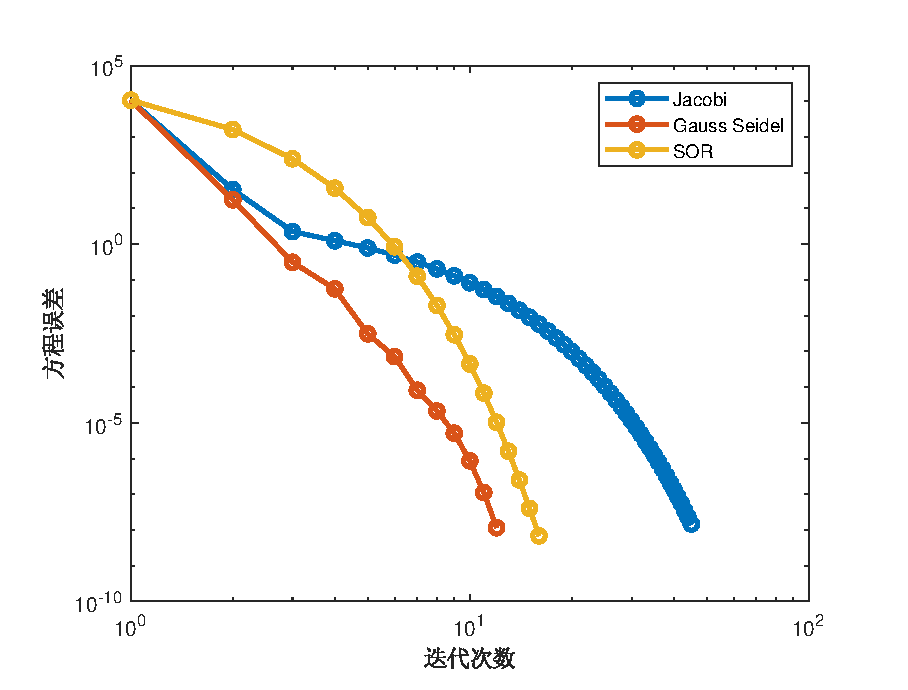
\includegraphics[width=0.45\textwidth]{1000_three_method.eps}
        \label{fig:image1}
    }
    \quad % Adjust horizontal space between images
    \subfloat[$n=10000$]{
        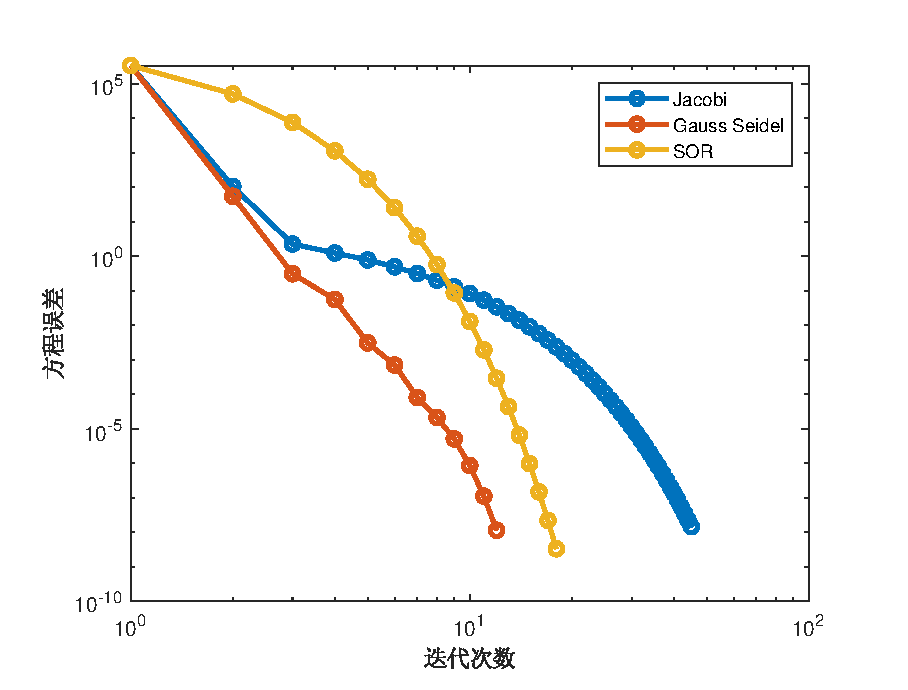
\includegraphics[width=0.45\textwidth]{10000_three_method.eps}
        \label{fig:image2}
    }
    \caption{误差(本文中误差均为后向误差)与迭代次数的关系}
    \label{fig:11}
\end{figure}

从图\ref{fig:11}可以看出,无论是 $n=1000$ 还是 $n=10000$ 的情况,Gauss Seidel 方法收敛速度都是最快的,SOR 方法在前期要比 Jacobi 方法差,但在完成前几次迭代后,迅速地超越了 Jacobi 方法.

Gauss Seidel 方法要好于 Jacobi 方法这是符合我们预期的,因为Gauss Seidel 迭代法每次迭代使用最新的变量值,故能够更快地逼近解.然而 SOR 方法比 Gauss Seidel 方法差这可能与 $\omega$ 的取值有关,因此,我们针对 $\omega$ 的取值对 SOR 迭代次数的影响展开实验:在 0.05到0.95中等距的取值并复制给 $\omega$,针对不同的 $\omega$ 分别计算算法收敛需要的迭代次数.其中,程序终止迭代的要求为误差小于等于 $10^{-8}$.
\begin{figure}[htbp]
    \centering
    \subfloat[松弛因子对收敛速度的影响]{
        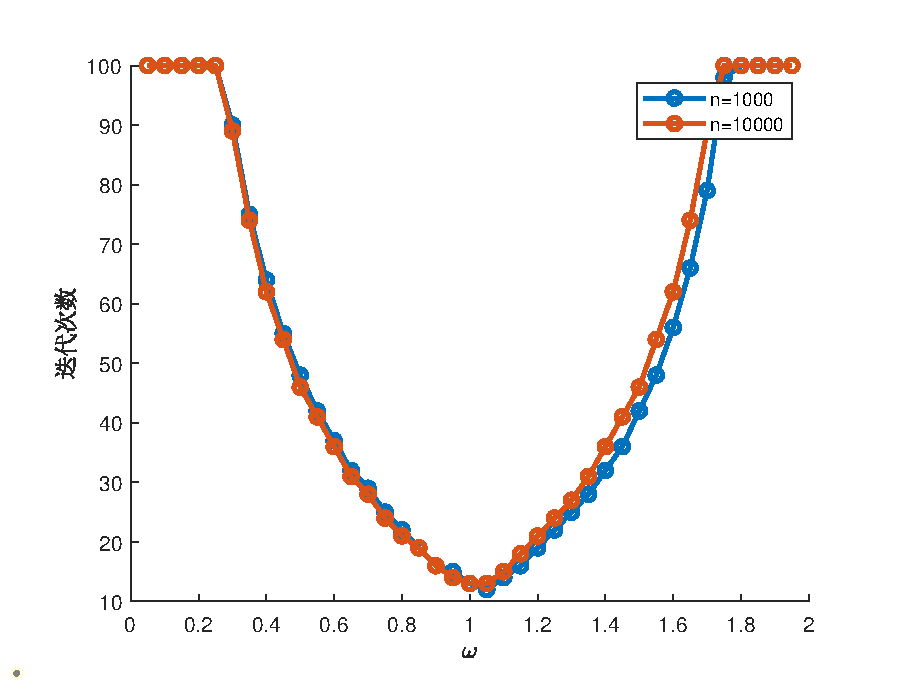
\includegraphics[width=0.45\textwidth]{omega.eps}
        \label{fig:omgea}
    }
    \quad % Adjust horizontal space between images
    \subfloat[$n=10000$]{
        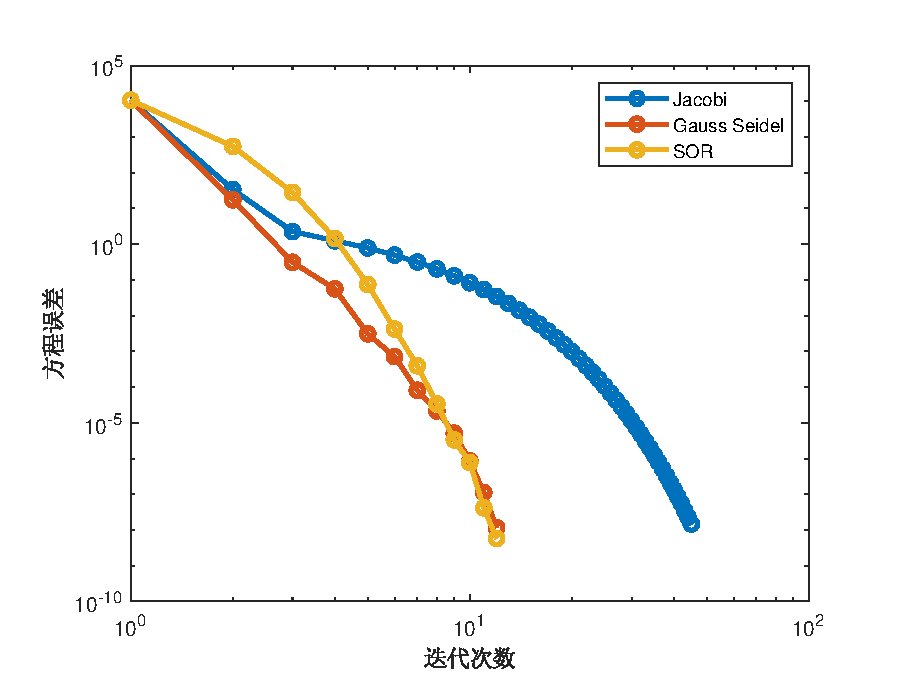
\includegraphics[width=0.45\textwidth]{105_three_method.eps}
        \label{fig:bestCompare}
    }
    \caption{误差(本文中误差均为后向误差)与迭代次数的关系}
    \label{fig:sidebyside}
\end{figure}
从图\ref{fig:omgea}中可以看出,SOR 方法的最优取值大约在 1到1.05之间,我们以 $\omega=1.05$ 重新比较三种方法.三种方法的收敛速度见图\ref{fig:bestCompare},可见当 $\omega$ 取值合理时,SOR 方法在临近收敛前要略好于 Gauss Seidel 方法.遗憾的是,无法针对所有问题给出一个通用的 $\omega$ 的取值.

\begin{proposition}
    虽然Jacobi方法收敛速度要远远慢于其他两种方法,但是由于 Jacobi 方法其计算顺序的没有依赖性,公式\eqref{equ:jacobi}中的$\bm{D}$矩阵由于其是对角矩阵,因此其取逆只需要对对角元素取对数即可.于是我们可以使用 MATLAB 的并行的矩阵乘法来加速计算.然而高斯赛德尔方法和SOR方法如果也想使用矩阵乘法的方式来进行迭代,需要计算 $D+L$ 和 $D+\omega L$ 的逆,这并不是一件容易的事情.因此后两种方法只能使用逐行逐列的方法,逐个更新每一个分量.所以在MATLAB实际计算中,Jacobi 方法反而是最快的方法.
\end{proposition}

\section{共轭梯度方法与预条件技术}
\begin{itemize}
    \item 共轭梯度方法
          共轭梯度方法在每一步中更新三个向量. 向量  $x_{k}$  是第  $k$  步时的近似解. 向量  $r_{k}$  表示近似解  $x_{k}$  的余项, $r_{k}=b-A x_{k}$. 变量  $d_{k}$  表示用于更新  $x_{k}$  得到改进的  $x_{k+1}$  时所使用的新的搜索方向. 算法的伪代码为:
          \begin{algorithm}
              \caption{Conjugate Gradient Method}
              \begin{algorithmic}[1]
                  \STATE $x_0 \gets \text{初始估计}$
                  \STATE $d_0 \gets r_0 \gets b - A x_0$
                  \FOR{$k = 0, 1, 2, \ldots, n - 1$}
                  \IF{$r_k = 0$}
                  \STATE stop, end
                  \ENDIF
                  \STATE $\alpha_k \gets \frac{r_k^T r_k}{d_k^T A d_k}$
                  \STATE $x_{k+1} \gets x_k + \alpha_k d_k$
                  \STATE $r_{k+1} \gets r_k - \alpha_k A d_k$
                  \STATE $\beta_k \gets \frac{r_{k+1}^T r_{k+1}}{r_k^T r_k}$
                  \STATE $d_{k+1} \gets r_{k+1} + \beta_k d_k$
                  \ENDFOR
              \end{algorithmic}
          \end{algorithm}

          该方法能够成功的原因在于所有的余项都和前面的余项正交. 如果能做到所有的余项正交, 该方法搜索所有的正交方向, 在经过至多  $n$  步就可以得到余项为零的正确解. 实现所有余项的正交的关键在于选择搜索方向  $d_{k}$ , 并使之两两共轭. 共轭的概念推广了正交的概念, 并据此在算法的名字中也包含“共轭”.
    \item  预条件技术

          在迭代求解线性方程组时,预条件技术(Preconditioning)是一种重要的方法,旨在通过改变原始问题的性质,提高迭代算法的收敛速度.预条件技术通过将线性方程组 \( Ax = b \) 转换为一个等价但更容易求解的问题:
          \begin{equation}
              M^{-1} A x = M^{-1} b
          \end{equation}
          其中,\( M \) 是预条件矩阵,通常选择 \( M \approx A \),但 \( M \) 应该易于求逆.理想的预条件矩阵能够减少 \( A \) 的条件数,从而加速迭代收敛.本次我们使用Jacobi 预条件:选择 \( M \) 为 \( A \) 的对角部分,即 \( M = \text{diag}(A) \).这种方法实现简单,并且可以有效提升梯度下降算法的收敛速度.
\end{itemize}

\begin{figure}[htbp]
    \centering
    \subfloat[$n=1000$]{
        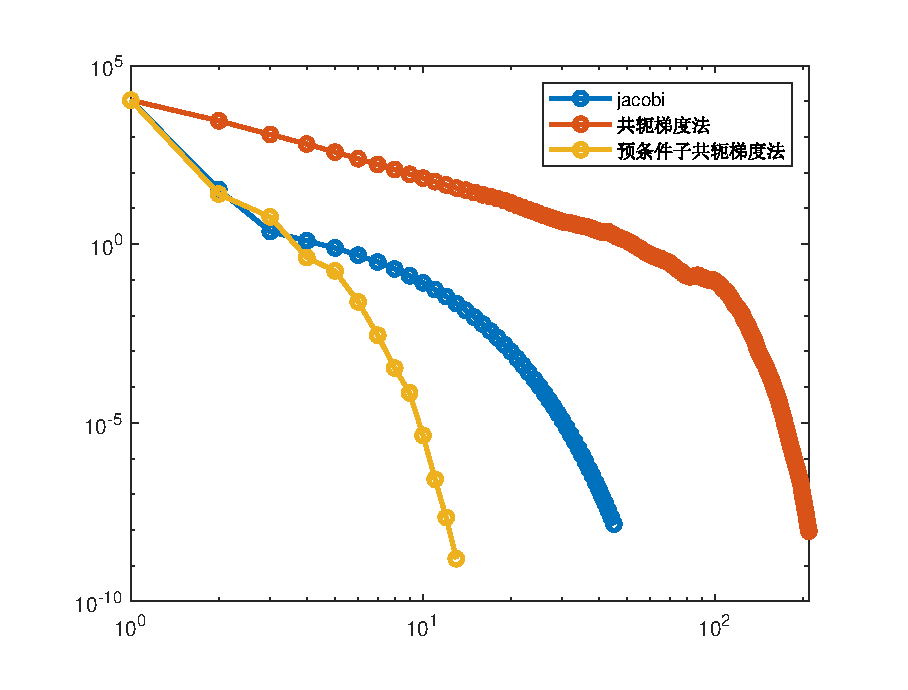
\includegraphics[width=0.45\textwidth]{1000_CG.eps}
        \label{fig:image1}
    }
    \quad % Adjust horizontal space between images
    \subfloat[$n=10000$]{
        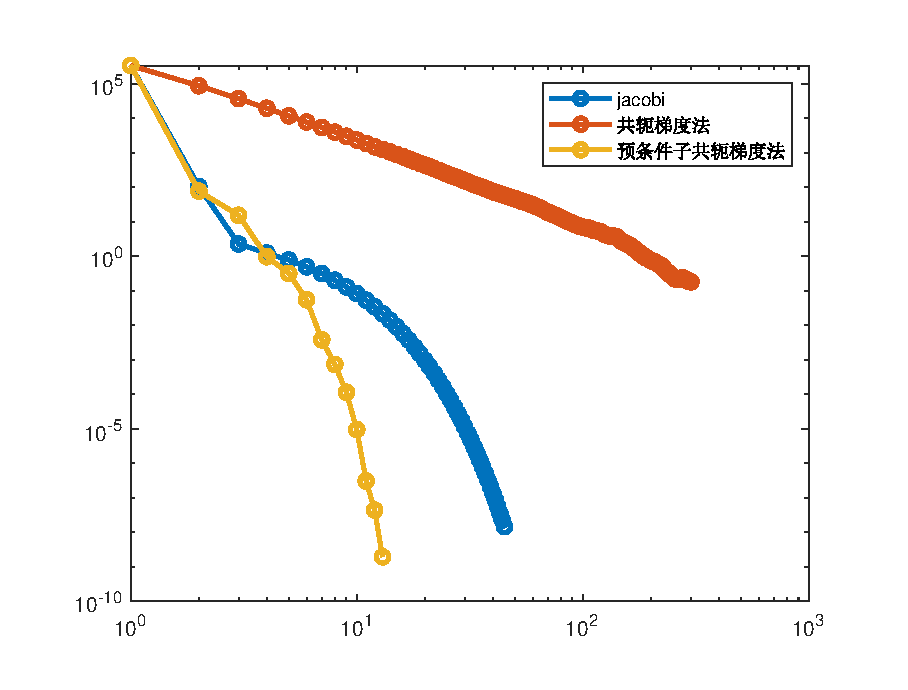
\includegraphics[width=0.45\textwidth]{10000_CG.eps}
        \label{fig:image2}
    }
    \caption{迭代次数与误差的关系}
    \label{fig:condition}
\end{figure}
我们分别比较了jacobi方法,共轭梯度法与预条件子共轭梯度法,同样对1000阶和10000阶的方程进行测试.图\ref{fig:condition}中可以看出在不加预条件子的情况下,共轭梯度法收敛速度非常慢,对于10000阶的情况几乎无法处理.预条件子技术大大的提升了共轭梯度法的收敛速度.

在最后,我们对更加困难的方案 $n=1e7$ 展开测试,此时矩阵过于庞大,需要使用稀疏矩阵技术减少内存消耗.此外,条件数达到了 $1.7425e+07$, 这给求解带来了很大的困难.使用了 Jacobi 预条件子进行求解,迭代次数 13 次,用时 16.74 秒,误差 $||Ax-b||_2=3.6479e-06$,$||Ax-b||_\infty = 9.3132e-09$.虽然13次就已经实现了比较好的效果,但是继续迭代已经无法使计算结果更好了.对于 $n=1e8$ 的情况,在创建矩阵 $A$ 时,即使使用稀疏矩阵计算机也会发生崩溃.总的来说,预条件子梯度下降法对于正定对称矩阵具有很好的求解效果.
\section{迭代方法的优势}
\begin{itemize}
    \item 虽然直接求解方法如高斯消元法在理论上可以求出方程的解析解,但是由于机器误差的存在,最后的计算结果仍然是有误差的.而迭代方法通过不断的迭代同样可以逼近机器精度.所以迭代求解方法的计算准确度是不比直接求解方法差的.
    \item 在实际生产实践中,对于解的精度要求并没有很高.迭代求解方法可以根据精度的要求提前终止迭代,从而加速计算.而直接计算方法如果提前结束计算就无法得到一个可用的解.
    \item 当 $A$ 或 $b$ 发生微小变化时,迭代求解方法可以直接使用上一次的系数计算出的解作为本次迭代的初始解,从而只需要很少的次数就可以收敛.而直接求解方法难以利用上次得到的计算结果,仍需要重新计算.
    \item 由于稀疏矩阵求解可以采用特殊的数据结构,所以计算机内存中可以储存相当大的稀疏矩阵.然而,如果采用直接求解算法,往往会破坏稀疏矩阵的结构,使其不再稀疏,这会给矩阵的储存带来很大的压力,甚至无法继续计算.迭代求解算法可以避免这个问题.
\end{itemize}


\clearpage
\begin{appendices}
    \section{MATLAB代码}
    \lstinputlisting[caption={\bf jacobi.m},]{savecode/jacobi.m}
    \lstinputlisting[caption={\bf gauss\_seidel.m},]{savecode/gauss\_seidel.m}
    \lstinputlisting[caption={\bf sor.m},]{savecode/sor.m}
    \lstinputlisting[caption={\bf preconditioned\_conjugate\_gradient.m},]{savecode/preconditioned\_conjugate\_gradient.m}
\end{appendices}
\end{document}